% Created 2023-11-26 Sun 13:38
% Intended LaTeX compiler: pdflatex
\documentclass[11pt]{article}
\usepackage[utf8]{inputenc}
\usepackage[T1]{fontenc}
\usepackage{graphicx}
\usepackage{longtable}
\usepackage{wrapfig}
\usepackage{rotating}
\usepackage[normalem]{ulem}
\usepackage{amsmath}
\usepackage{amssymb}
\usepackage{capt-of}
\usepackage{hyperref}
\usepackage[margin=0.5in]{geometry}
\author{Agustín Alejandro Mota Hinojosa}
\date{\today}
\title{PL/SQL 6-5}
\hypersetup{
 pdfauthor={Agustín Alejandro Mota Hinojosa},
 pdftitle={PL/SQL 6-5},
 pdfkeywords={},
 pdfsubject={},
 pdfcreator={Emacs 29.1 (Org mode 9.7)}, 
 pdflang={English}}
\begin{document}

\maketitle
\tableofcontents

\section{Vocabulary}
\label{sec:orgb6baa31}

FOR UPDATE Declares that each row is locked as it is being fetched so other users cannot modify the rows while the cursor is open
NOWAIT A keyword used to tell the Oracle server not to wait if the requested rows have already been locked by another user
\section{Try It / Solve It}
\label{sec:org6f8e60c}
In this Practice you will INSERT and later UPDATE rows in a new table: PROPOSED\textsubscript{RAISES}, which will store details of salary increases proposed for suitable employees. Create this table by executing the following SQL statement:

\begin{verbatim}
CREATE TABLE proposed_raises
(date_proposed DATE,
date_approved DATE,
employee_id NUMBER(6),
department_id NUMBER(4),
original_salary NUMBER(8,2),
proposed_new_salary NUMBER(8,2));
\end{verbatim}
\begin{enumerate}
\item Write a PL/SQL block that inserts a row into PROPOSED\textsubscript{RAISES} for each eligible employee. The eligible employees are those whose salary is below a chosen value. The salary value is passed as a parameter to the cursor. For each eligible employee, insert a row into PROPOSED\textsubscript{RAISES} with date\textsubscript{proposed} = today’s date, date\textsubscript{appoved} null, and proposed\textsubscript{new}\textsubscript{salary} 5\% greater than the current salary. The cursor should LOCK the employees rows so that no one can modify the employee data while the cursor is open. Test your code using a chosen salary value of 5000.
\begin{verbatim}
DECLARE
    CURSOR cur_emp (chosen_salary NUMBER) IS (
        SELECT employee_id,salary,department_id FROM employees WHERE salary < chosen_salary
    );
    v_value NUMBER;
BEGIN
    v_value := 5000;
    FOR rec IN cur_emp(v_value) LOOP
        INSERT INTO proposed_raises
            (date_proposed, date_approved, employee_id, department_id,
                            original_salary, proposed_new_salary)
        VALUES
            (SYSDATE,null,rec.employee_id,rec.department_id,rec.salary,rec.salary * 1.5);
    END LOOP;
END;
\end{verbatim}
\item SELECT from the PROPOSED\textsubscript{RAISES} table to see the results of your INSERT statements. There should be 15 rows. If you run your block in question 1 more than once, make sure the PROPOSED\textsubscript{RAISES} table is empty before each test.
\begin{verbatim}
 SELECT * FROM proposed_raises;
 DELETE FROM proposed_raises; -- to clear all rows from the table
\end{verbatim}

\begin{center}
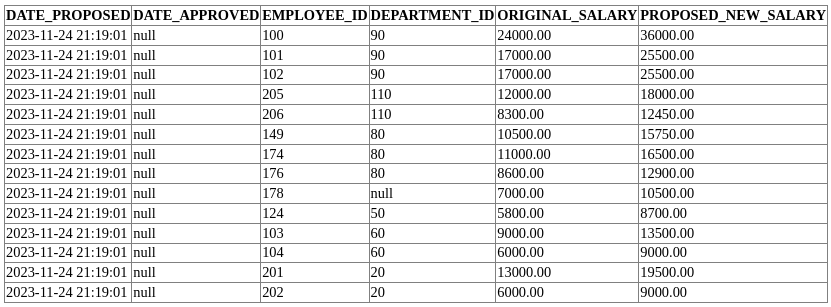
\includegraphics[width=.9\linewidth]{./resources/prop_sal_tab1.png}
\end{center}

\item Imagine these proposed salary increases have been approved by company management.
\begin{enumerate}
\item Write and execute a PL/SQL block to read each row from the \texttt{PROPOSED\_RAISES} table. For each row, UPDATE the \texttt{date\_approved} column with today’s date. Use the WHERE CURRENT OF\ldots{} syntax to UPDATE each row. After running your code, SELECT from the \texttt{PROPOSED\_RAISES} table to view the updated data.
\begin{verbatim}
DECLARE
    CURSOR cur_emp IS
        SELECT * FROM proposed_raises FOR UPDATE NOWAIT;
    v_emp_rec cur_emp%ROWTYPE;
BEGIN
    OPEN cur_emp;
    LOOP
        FETCH cur_emp INTO v_emp_rec;
        EXIT WHEN cur_emp%NOTFOUND;
        UPDATE proposed_raises
            SET date_approved = SYSDATE
        WHERE CURRENT OF cur_emp;
    END LOOP;
    CLOSE cur_emp;
END;
\end{verbatim}

\begin{center}
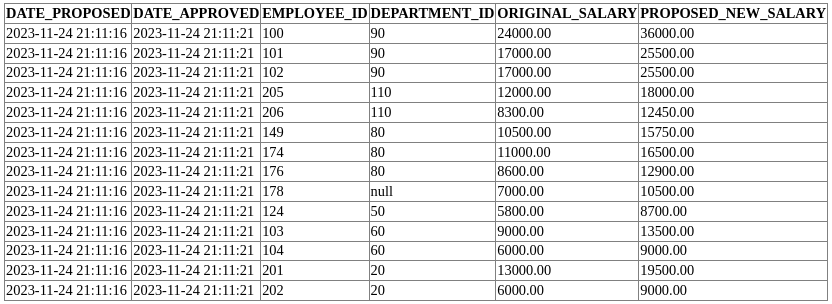
\includegraphics[width=.9\linewidth]{./resources/prop_sal_tab2.png}
\end{center}

\item Management has now decided that employees in department 50 cannot have a salary increase after all. Modify your code from question 3 to DELETE employees in department 50 from \texttt{PROPOSED\_RAISES}. This could be done by a simple DML statement (DELETE FROM \texttt{proposed\_raises} WHERE \texttt{department\_id} = 50;), but we want to do it using a FOR UPDATE cursor. Test your code, and view the \texttt{PROPOSED\_RAISES} table again to check that the rows have been deleted.
\begin{verbatim}
DECLARE
    CURSOR cur_emp IS
        SELECT *
            FROM proposed_raises
        WHERE department_id = 50 FOR UPDATE NOWAIT;
    v_emp_rec cur_emp%ROWTYPE;
BEGIN
    OPEN cur_emp;
    LOOP
        FETCH cur_emp INTO v_emp_rec;
        EXIT WHEN cur_emp%NOTFOUND;
        DELETE FROm proposed_raises WHERE CURRENT OF cur_emp;
    END LOOP;
    CLOSE cur_emp;
END;
\end{verbatim}
\end{enumerate}
\end{enumerate}
\end{document}